\chapter{Linked Lists}

A linked list is a linear data structure where each element is a
separate object, called a node. Each node holds its own data and the
address of the next node, thus forming a chain-like structure.\index{linked list}

A simple node in a linked list can be represented in C++ as follows:



\begin{lstlisting}[language=C++]
struct Node {
    int data;
    Node* next;
};
\end{lstlisting}

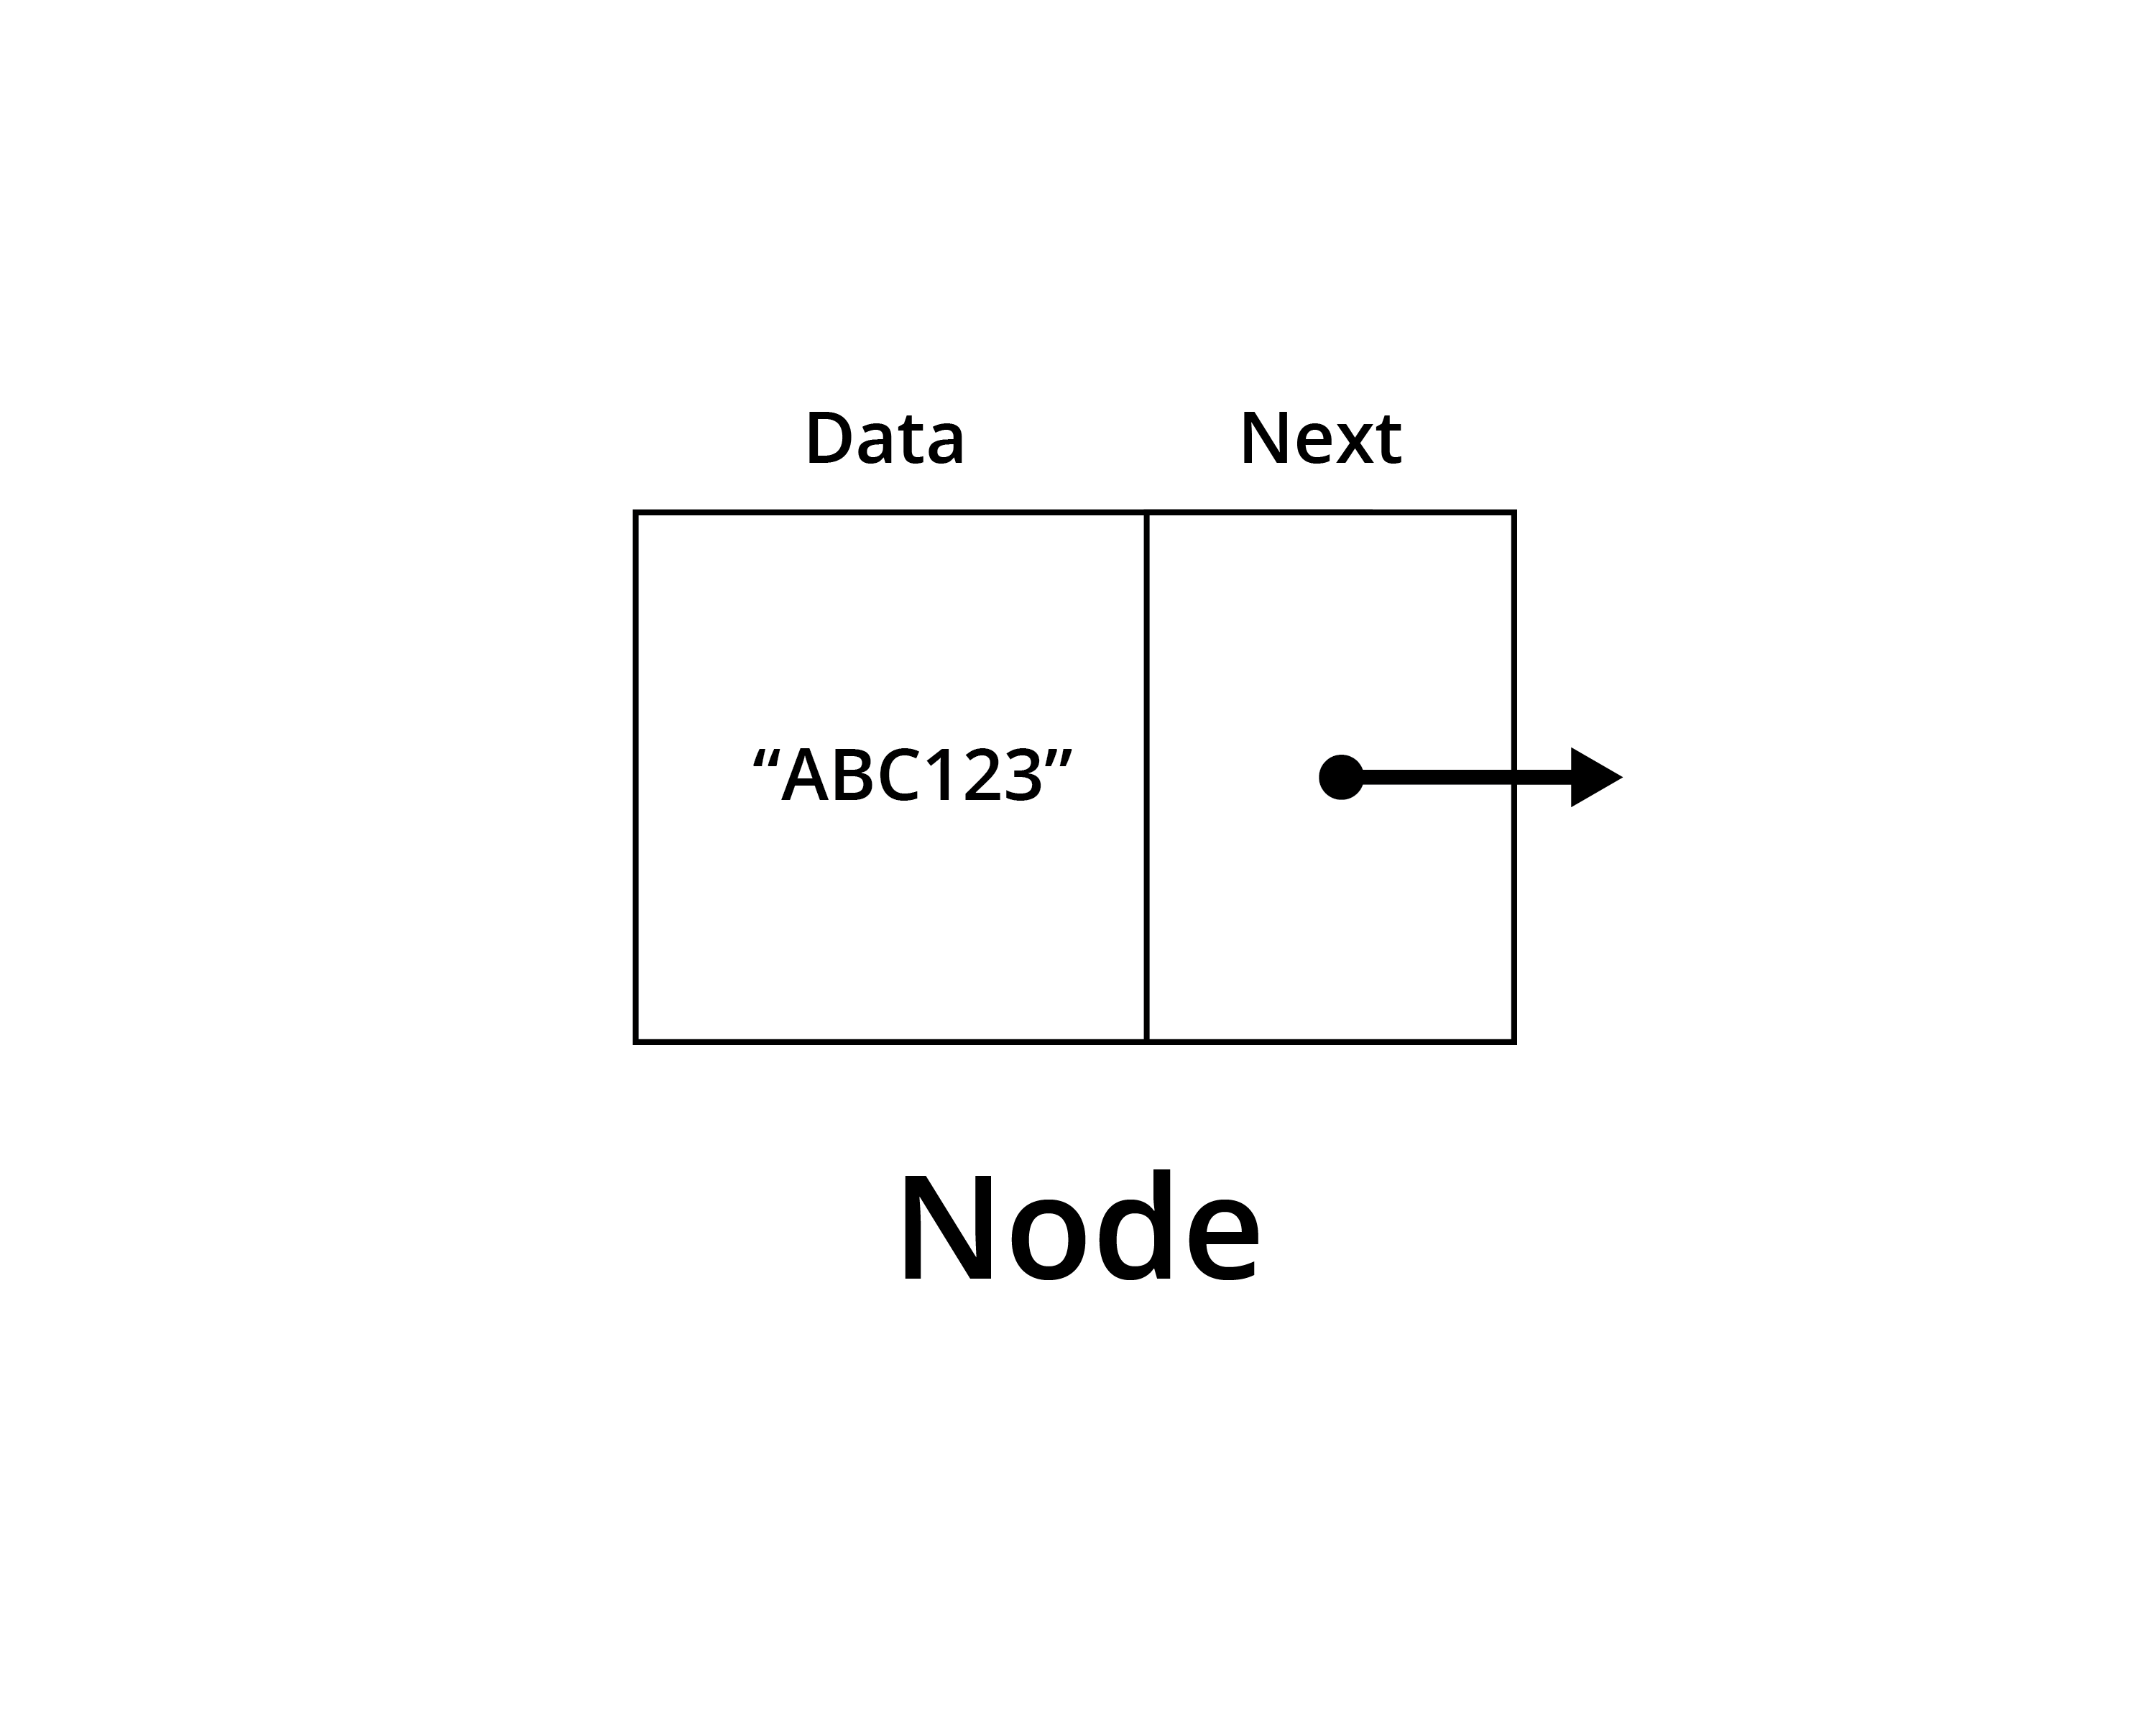
\includegraphics[width=0.5\textwidth]{node.png}


In this structure, 'data' is used to store the data and 'next' is a
pointer that holds the address of the next Node in the list.



Here is a simple example of creating and linking nodes in a linked
list:

\begin{lstlisting}[language=C++]
// Create nodes
Node* head = new Node();
Node* second = new Node();
Node* third = new Node();
\end{lstlisting}
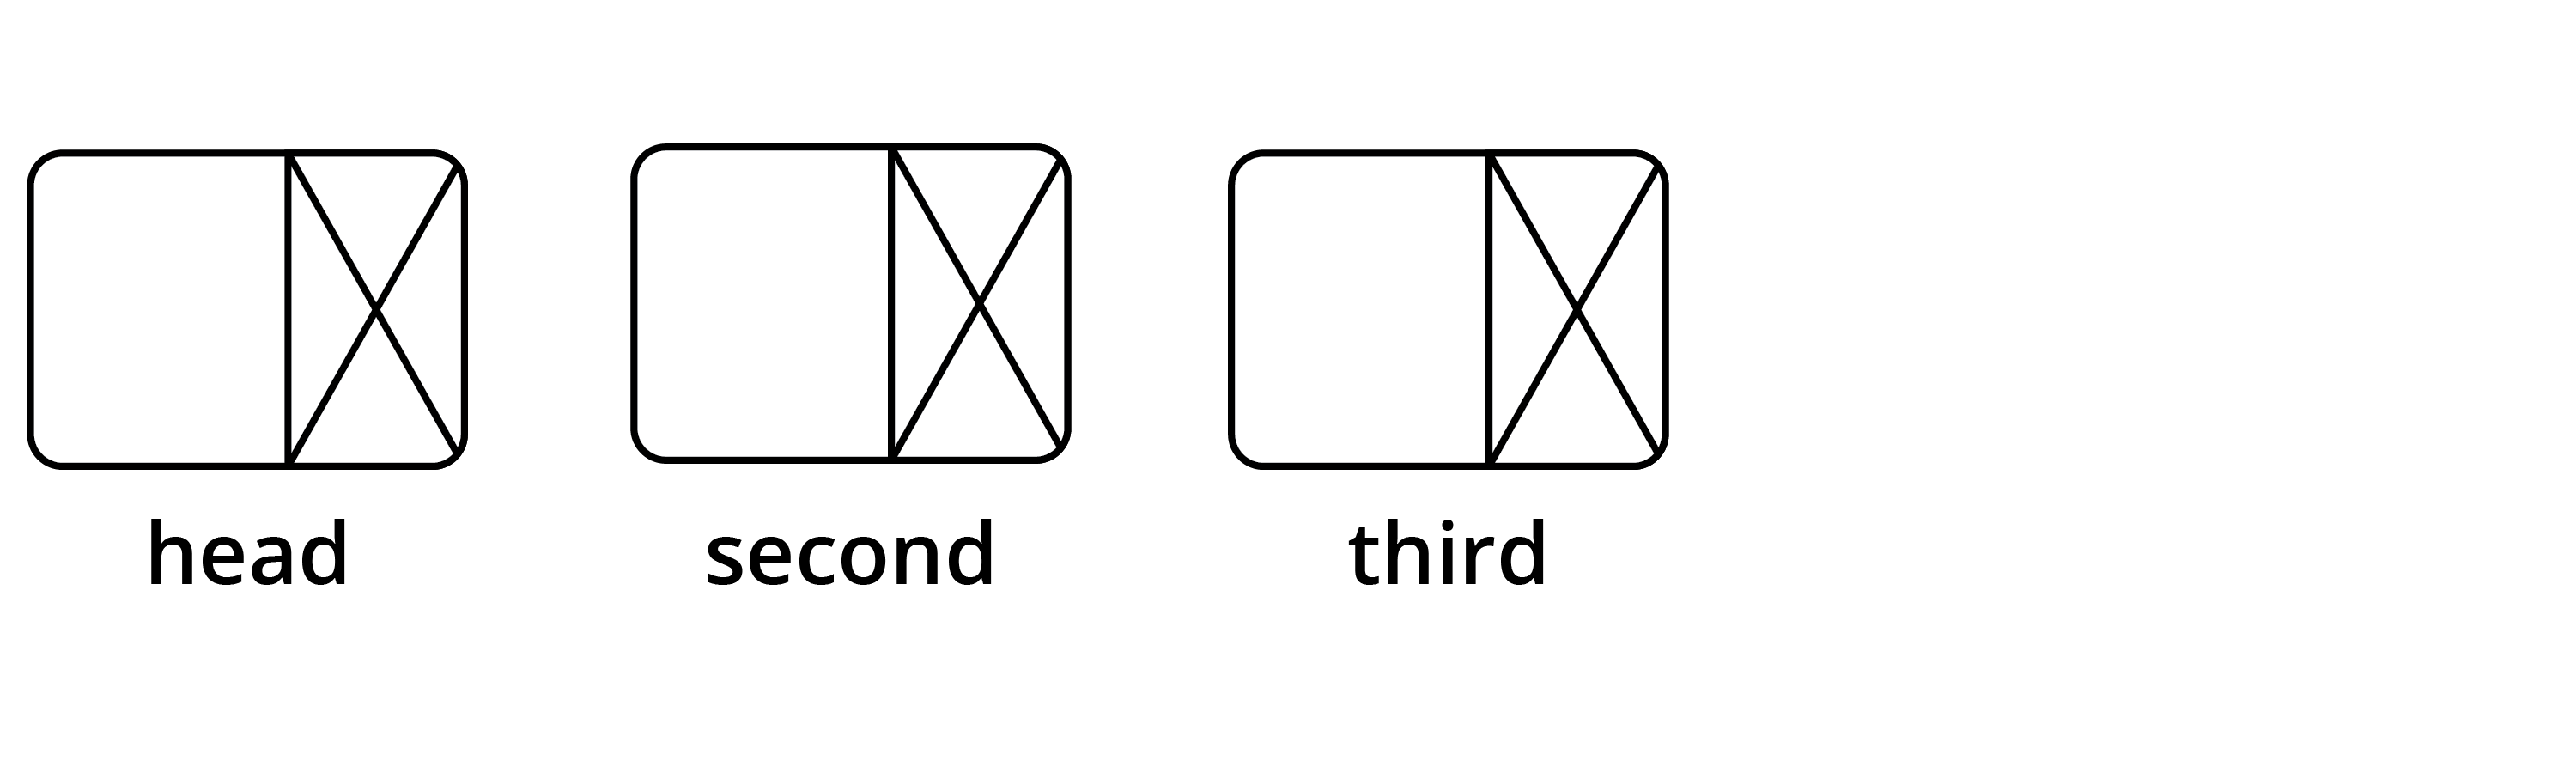
\includegraphics[width=.75\textwidth]{llexample-03.png}

\begin{lstlisting}[language=C++]

// Assign data
head->data = 1;
second->data = 2;
third->data = 3;
\end{lstlisting}

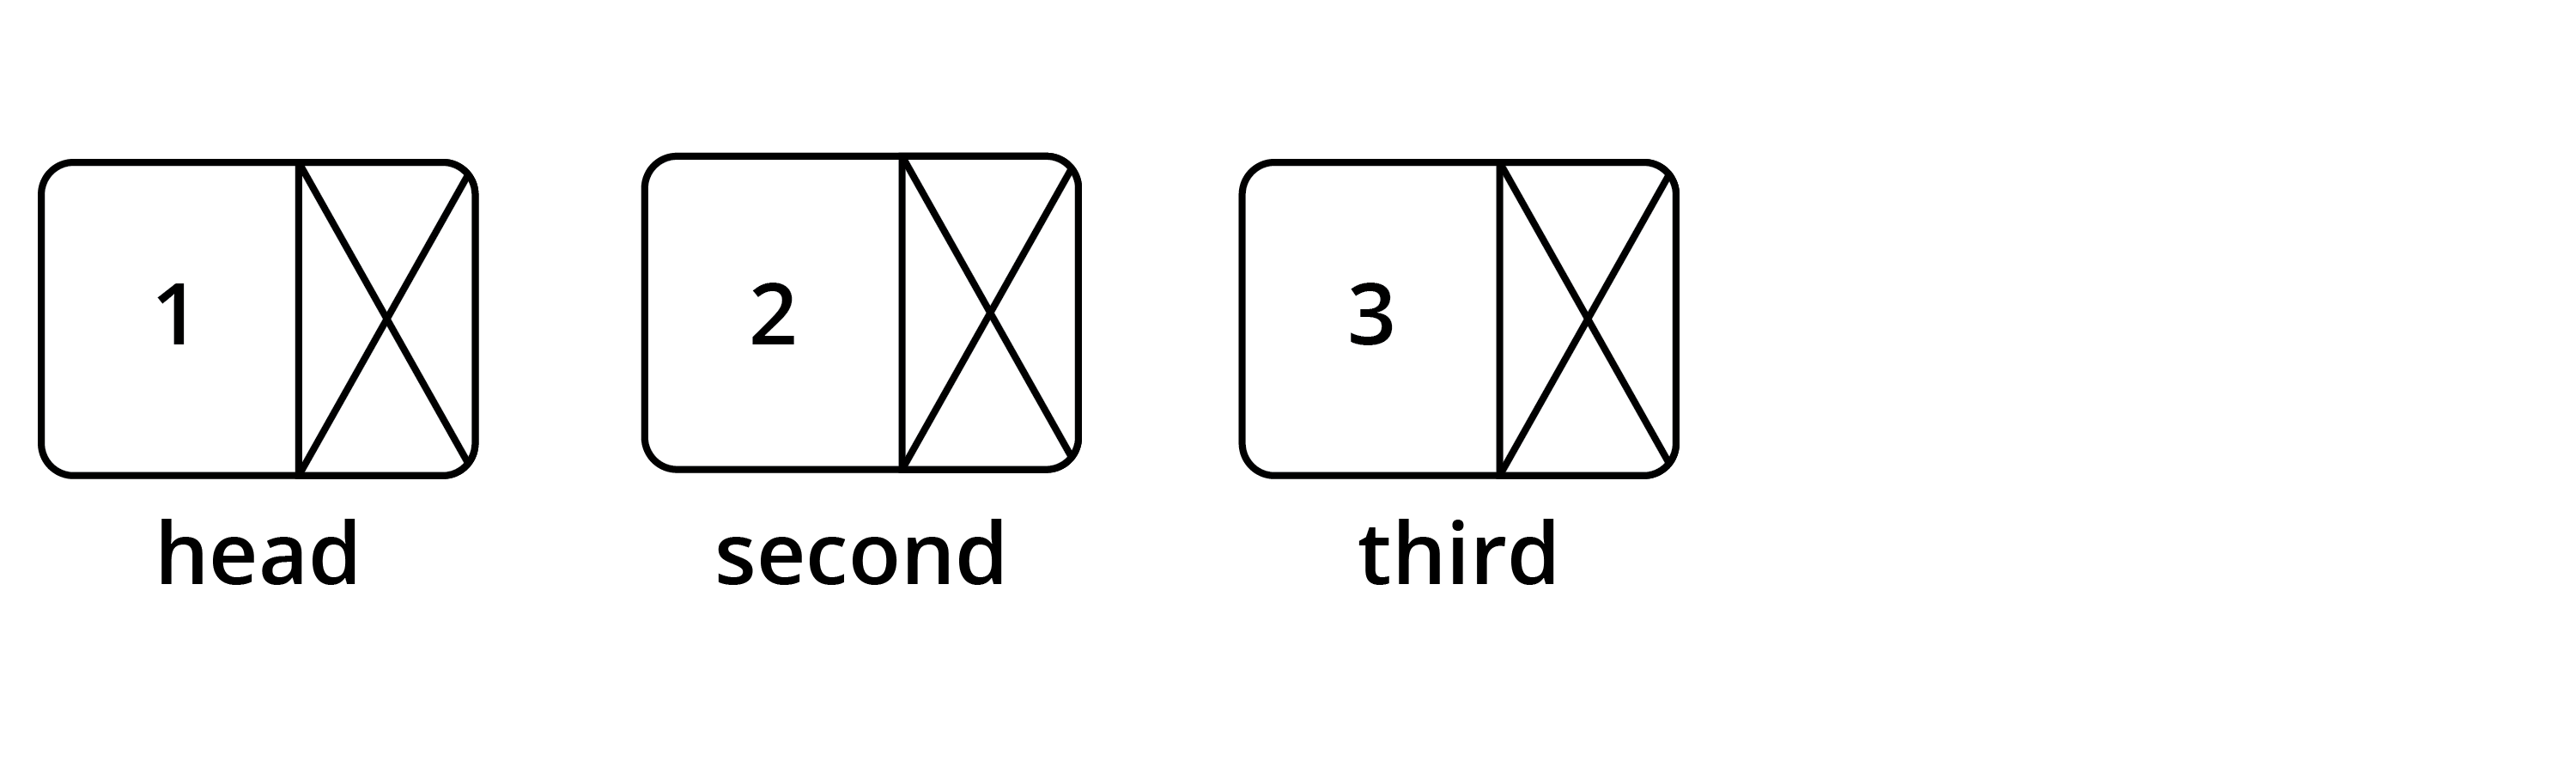
\includegraphics[width=.75\textwidth]{llexample-04.png}

\begin{lstlisting}[language=C++]
// Link nodes
head->next = second;
second->next = third;
third->next = nullptr;  // The last node points to null
\end{lstlisting}


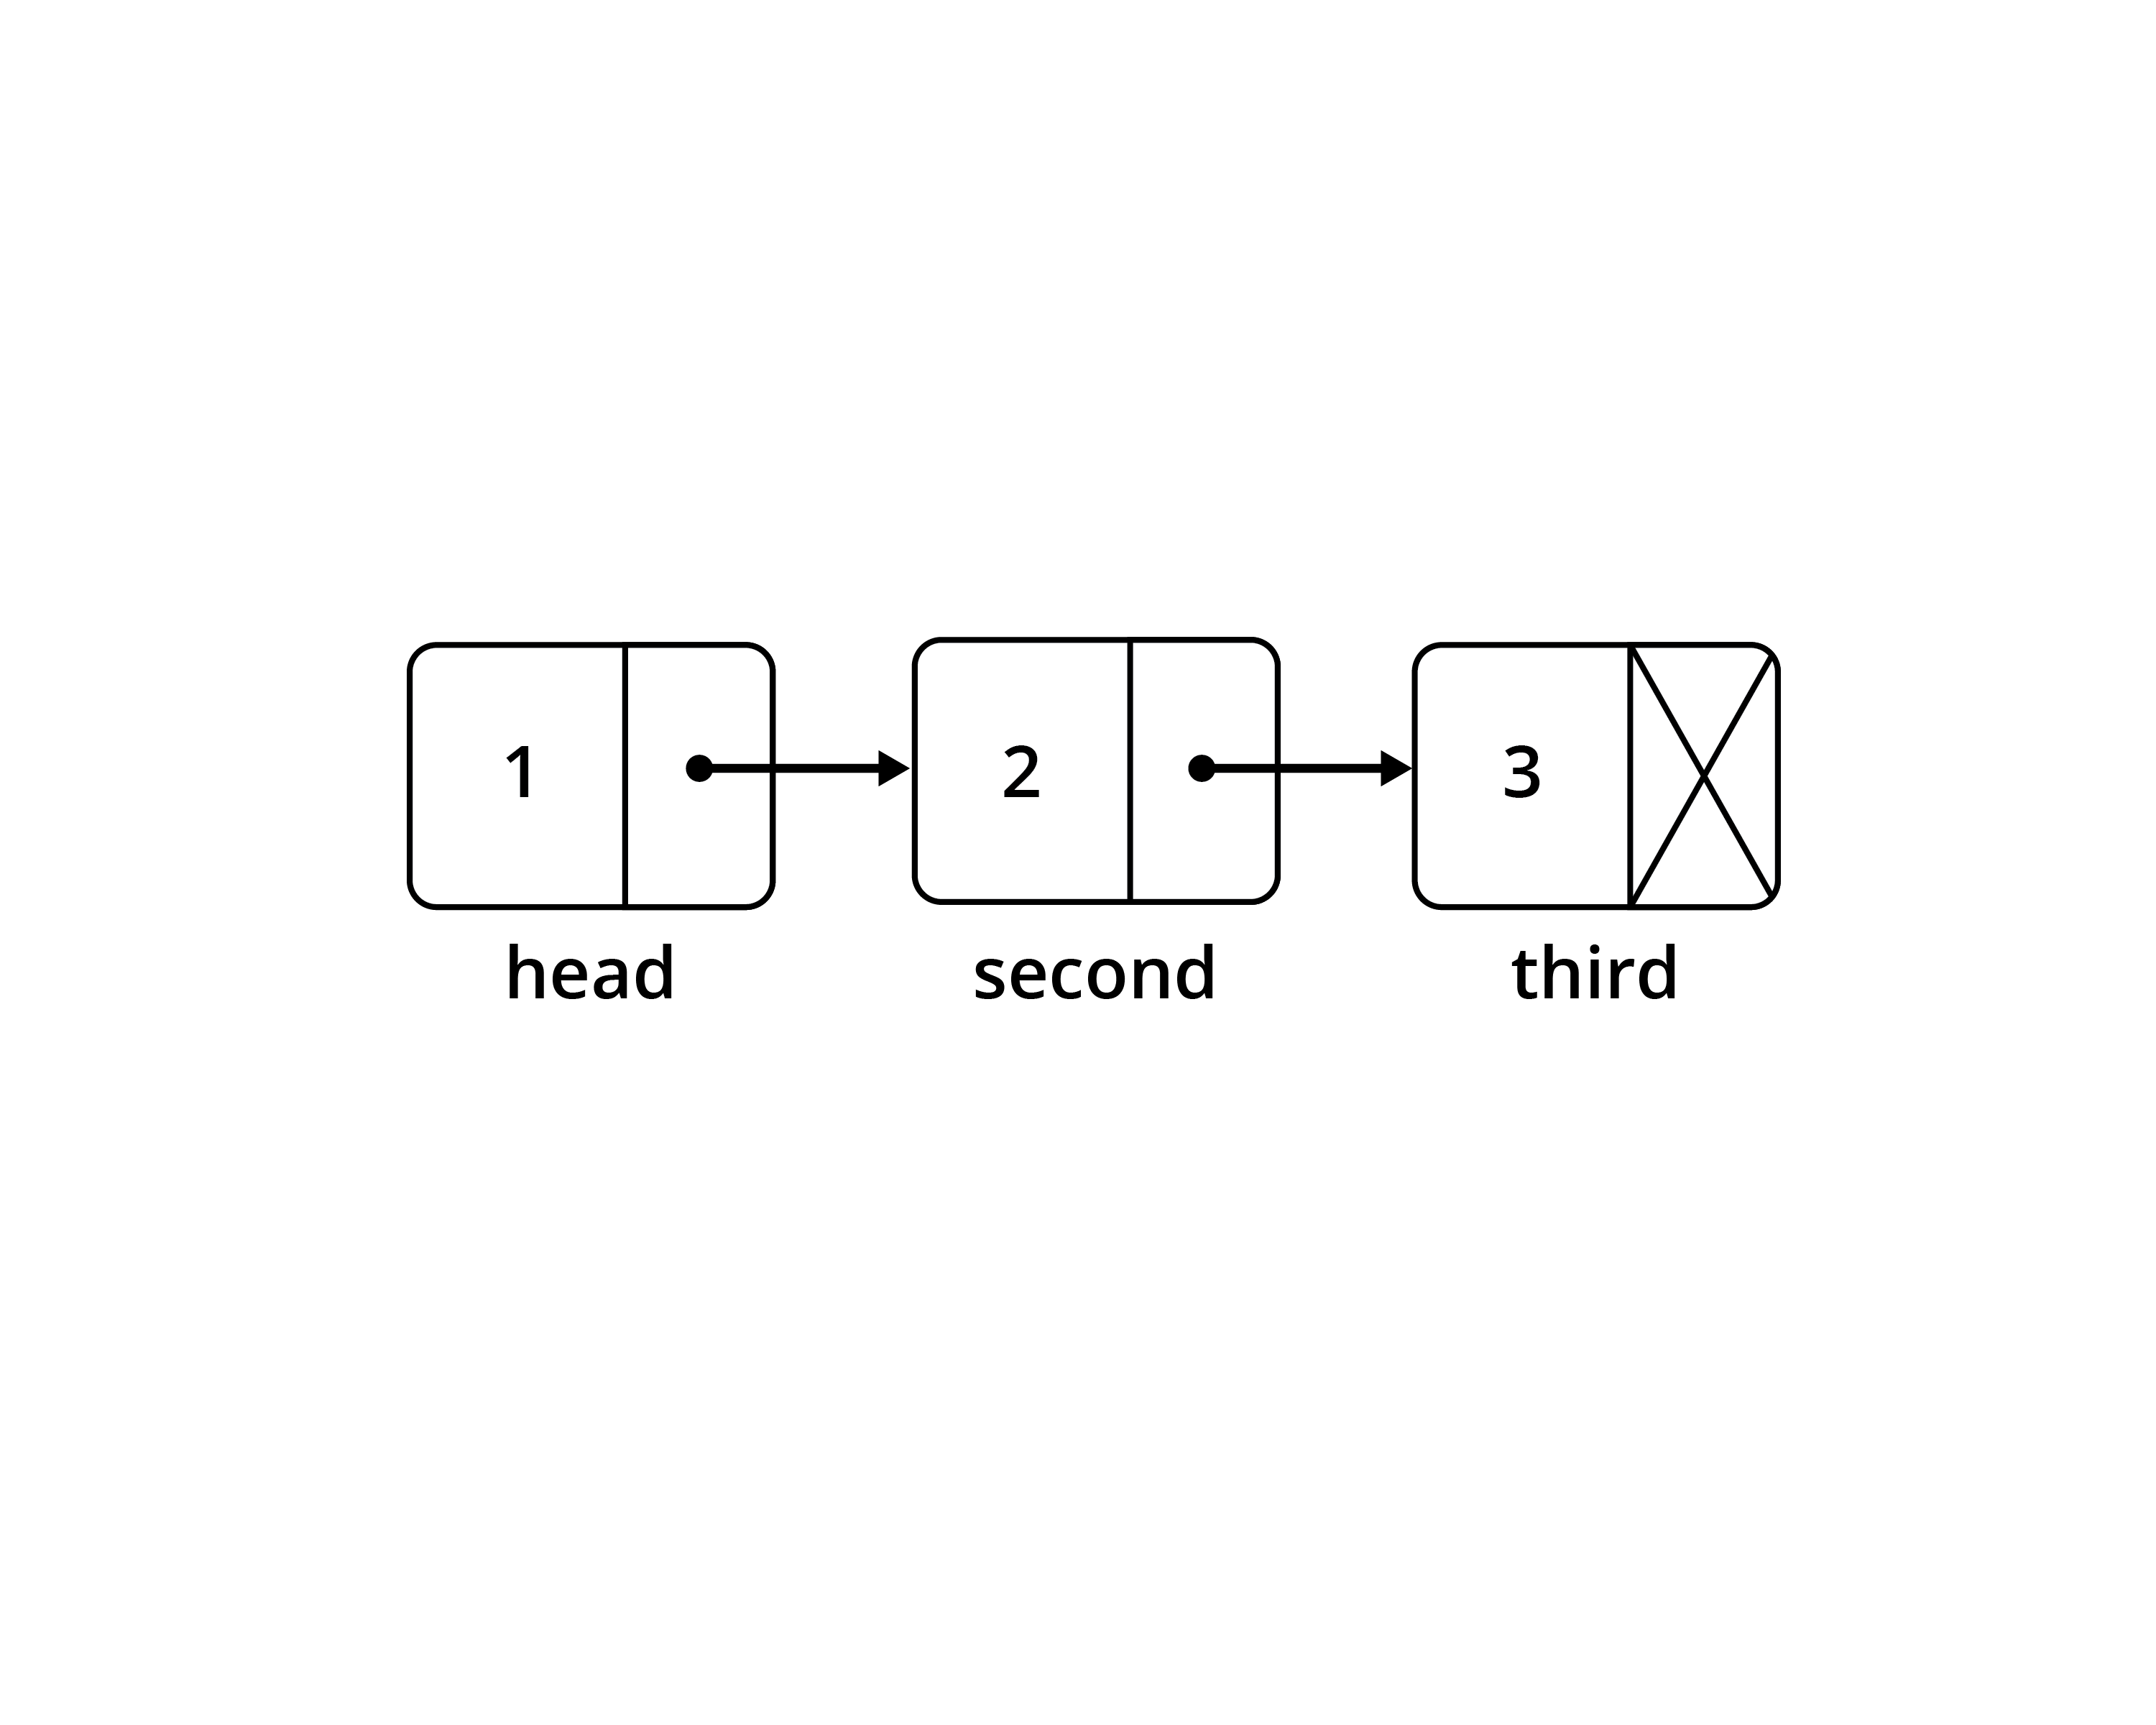
\includegraphics[width=.75\textwidth]{llexample-05.png}



In this example, we first create three nodes using the `new` keyword,
which dynamically allocates memory. We then assign data to the nodes
and link them using the 'next' pointer.

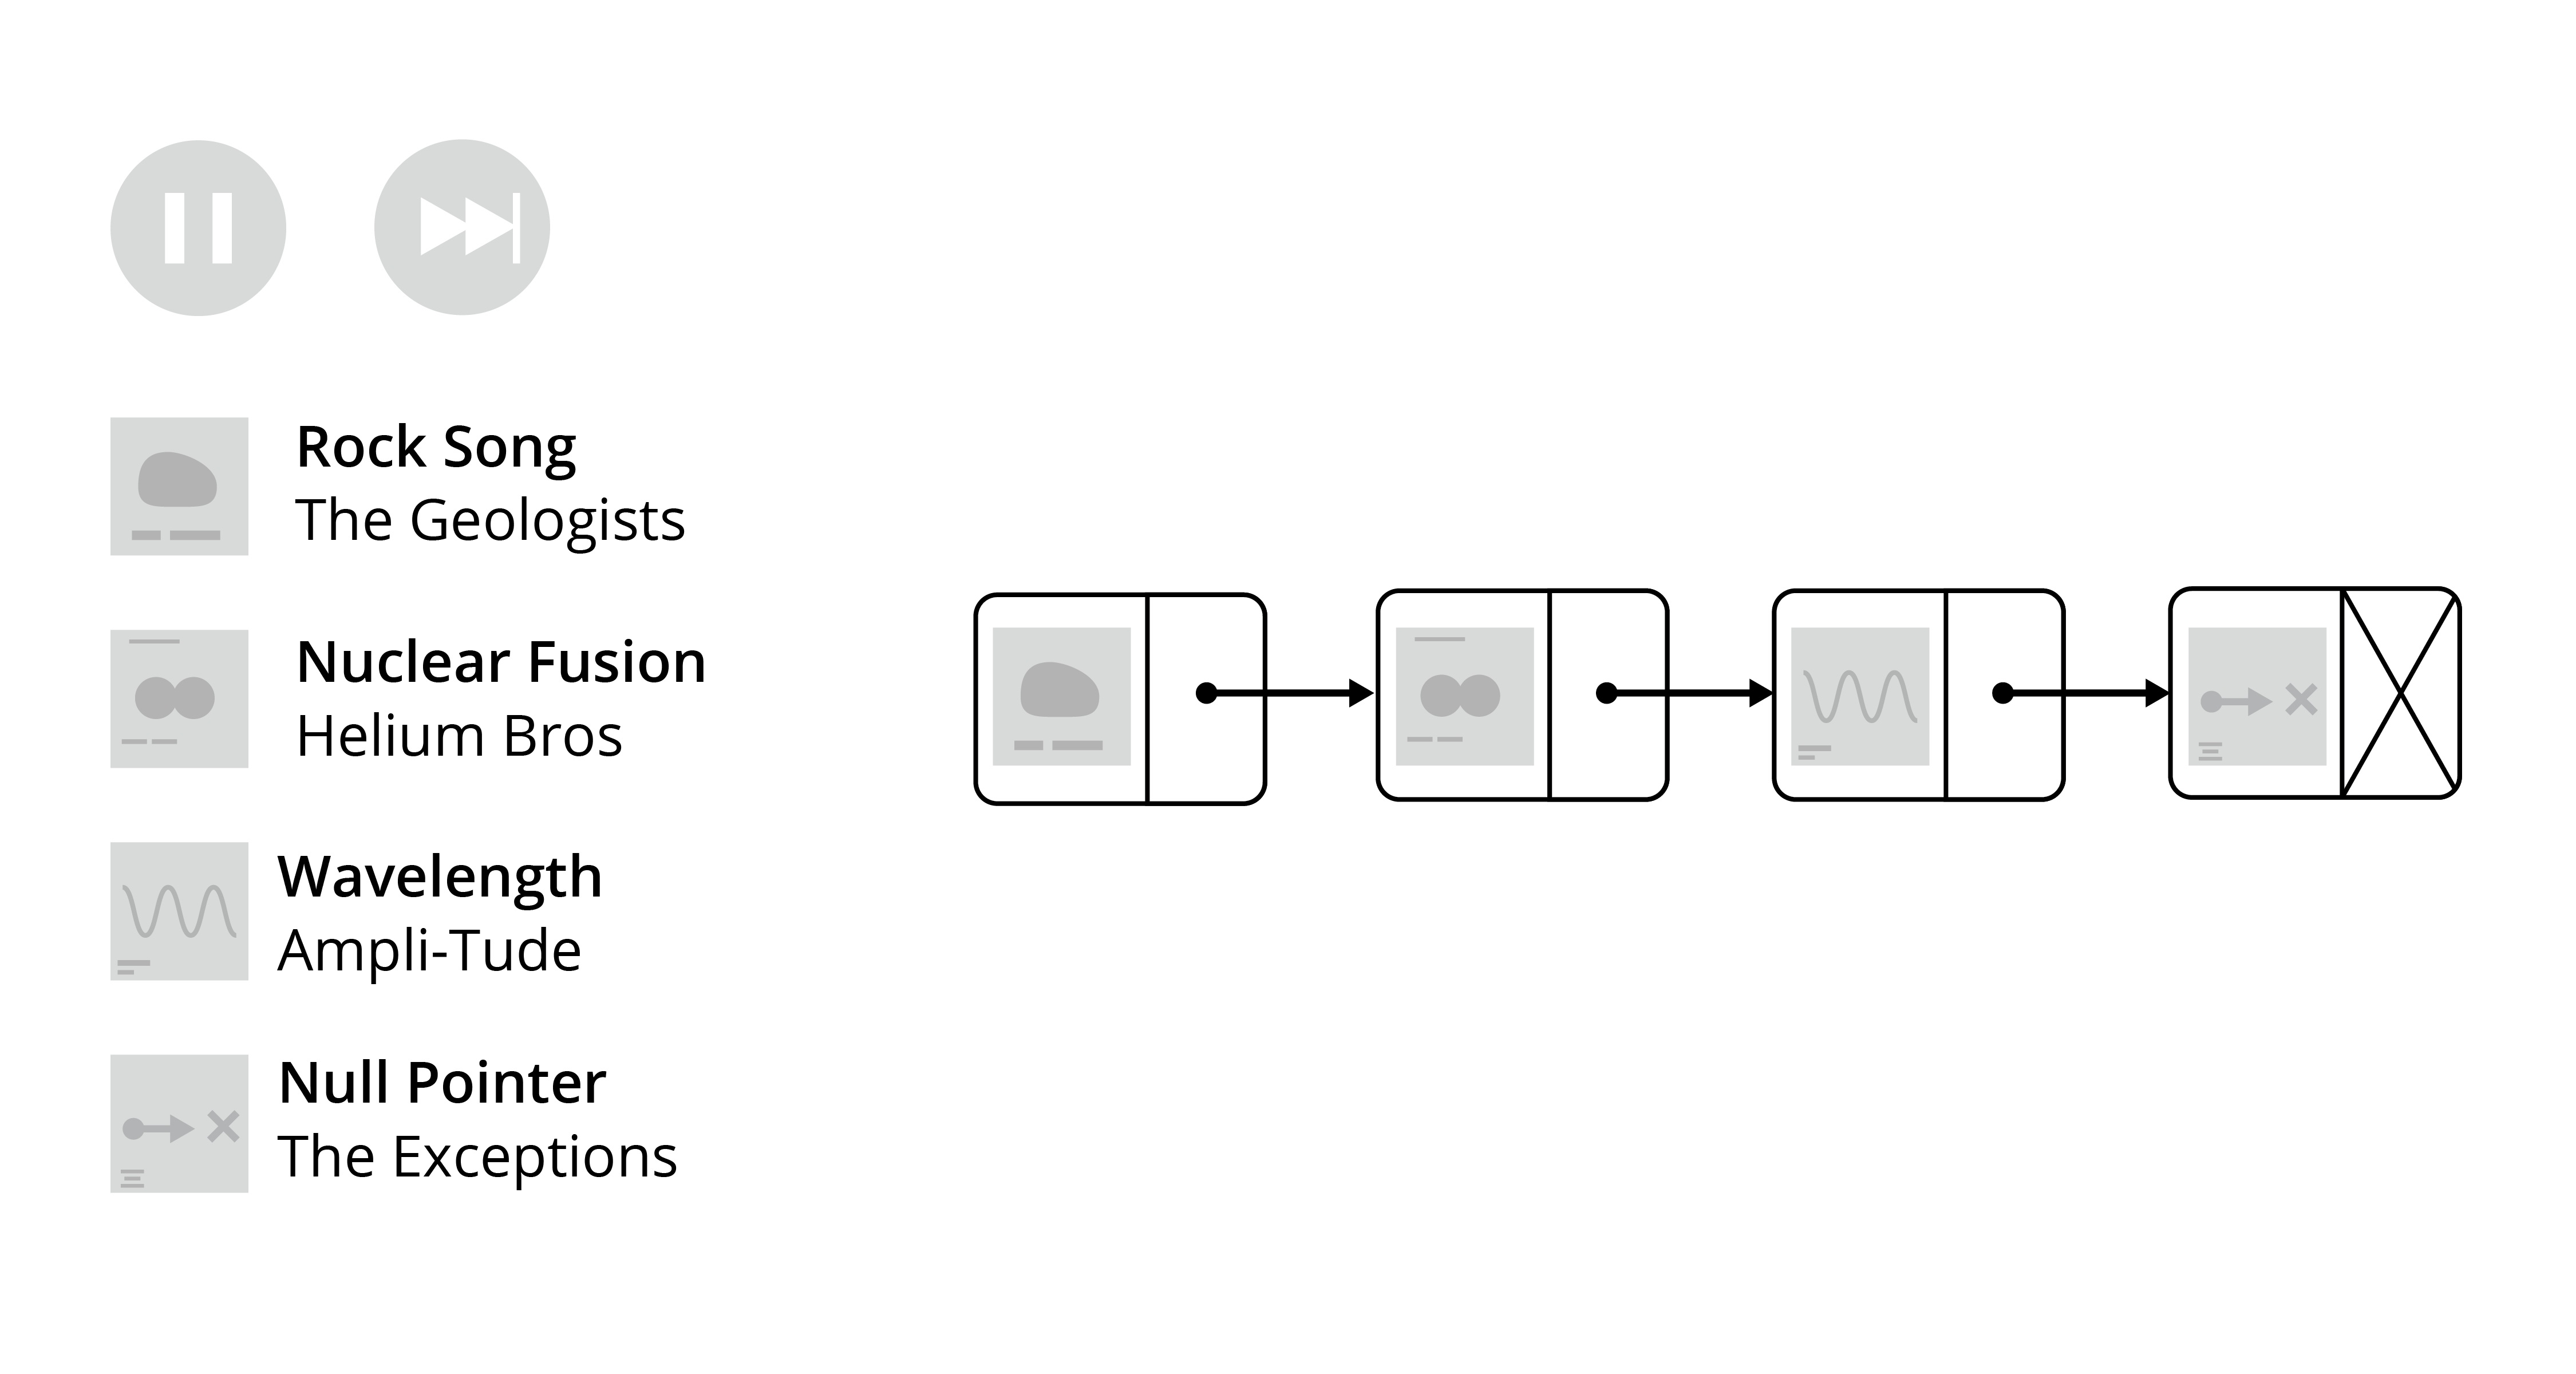
\includegraphics[width=1\textwidth]{playlistCombined.png}
